\documentclass[12pt,a4paper,twoside]{article}

\usepackage{fancyhdr}
\usepackage{lastpage}
\usepackage{a4wide}
\usepackage{alegreya}
\usepackage{amsmath}
\usepackage{amssymb}
\usepackage{float} 
\usepackage{graphicx}
\usepackage{hyperref}
\usepackage{color}
\usepackage{fancybox}
\usepackage{moreverb}
%\usepackage{hangcaption}
\usepackage{listings}
\usepackage{indentfirst}
\usepackage[utf8]{inputenc}
\usepackage[OT1]{fontenc}
\raggedbottom

%\fbox{}
%\shadowbox{}
%\doublebox{}
%\ovalbox{}
%\Ovalbox{}
%\shabox{}


% --- Logo Atos ---
%\makebox[\textwidth][l]{
%\raisebox{-15pt}[0pt][0pt]{
%\hspace{2.5cm}
%\includegraphics[scale=0.1]{Images/logo_atos.eps}
%}
%}
\title{2nd year intership report}
\author{Ramarijaona Maeva}
\date{\today}

\pagestyle{headings}

\begin{document}
\lstset{ numbers=left, tabsize=3, frame=single, numberstyle=\ttfamily, basicstyle=\footnotesize} 
\thispagestyle{empty}

\begin{center}
\makebox[\textwidth][l]{
\raisebox{-8pt}[0pt][0pt]{

\includegraphics[scale=0.40]{logo_solystic_north.jpg}
}
}
\makebox[\textwidth][r]{
\raisebox{0pt}[0pt][0pt]{

\includegraphics[scale=0.25]{logo_ensimag.pdf}
}
}
Grenoble INP  -- ENSIMAG\\
Ecole Nationale Superieure dInformatique et de Mathematiques Appliquees\\
\vspace{3cm}
{\LARGE Second year internship report}\\
\vspace{1cm}
At Solystic SAS\\
\vspace{2cm}
\shadowbox{
\begin{minipage}{1\textwidth}
\begin{center}
{\Huge Implementing a new architecture for a software suite integrated to the Information Systems inherent in the field of object sorting}\\
\end{center}
\end{minipage}
}\\
\vspace{3cm}
RAMARIJAONA Maeva\\
2nd year -- ISI Specialization\\
\vspace{3mm}
June 1st 2017 - September 13th 2017 (14 weeks)\\
\vspace{2cm}
% * <maeva.ramarijaona@gmail.com> 2017-09-09T11:08:59.941Z:
%
% ^.
% * <maeva.ramarijaona@gmail.com> 2017-09-09T11:08:58.293Z:
%
% ^.
\begin{tabular}{p{10cm}p{10cm}}
{\bf Solystic SAS}                                            &{\bf Internship supervisor}\\
{\footnotesize 21 rue de Chony}       & ~~~CROUZET Lionel\\
{\footnotesize BP 102}                                        & {\bf Ensimag Reviewer}\\
{\footnotesize 26501 BOURG LES VALENCE CEDEX}                          & ~~~?\\
\end{tabular}
\end{center}
\newpage
% \begin{abstract}
% Your abstract.
% \end{abstract}

\tableofcontents
\newpage
\section{Introduction}

\subsection{Company Overview}%TO-DO : complete this

Solysitc is a French company that is a wholly owned subsidiary of Northrop Grumman and specializes in mail sorting. It provides sorting, coding and reading systems used in mail sorting centers all around the world, softwares to help program and monitor these systems and assistance and maintenance of the systems in sorting sites. With more than 800 patents applications filed and 7\% of yearly spendings dedicated to R\&D, Solystic tries to accomodate the multiple needs of their diverse clientèle by constantly trying to improve the services they make available.

With clients in 28 countries and an average annual revenue of \$120M , Solystic is the leader company in the sector of mail sorting.

\subsection{Object of the mission : the SoMoS II application}

My internship was centered around modifying an already existing application called SoMoS II, developed in 2016 It is written in PHP and uses the Symfony framework, and usually deployed on an Apache server. This application was originally intended for use by BPost which is the Belgian postal service.

This application consists of three main parts : Administration, Data Management and Scenario Management. The Administration part is used to manage the production resources, which means the sorting systems, sorting sites and sorting parameters, as well as the user rights. The Data management part helps manage data from 2 different databases, AVCS and ROMA. Finally the Scenario part allows a user to create, view, edit, run or delete a scenario in order to simulate or predict the sorting and distribution of mail according to the production resources information provided by the other two parts.

\section{Dividing an application in services connected by a bus}
\subsection{A global architecture issue more than a problem with the particular application}
The SoMoS II application offers a range of useful functionalities and is practical for a client on its own. However, it is when associated with other applications that the current architecture shows some flaws. For instance, most of the functionalities seen in the Administration part are useful in other applications, yet those applications have no means to share these features with SoMoS II. That means they each have to have an implementation of these functionalities, and this poses an issue when an update is needed on any of these features, as all the applications have to be updated. This architecture also makes it difficult to upscale the services. Yet, for Solysitc's clients, upscaling is essential as sorting sites may change capacity over time and some house hundreds of systems that might each send thousands of requests each to these different services.

Building such monolithic and inter independent applications may ensure a sense of stability, indeed if an application crashes, the others are unaffected and a given functionality is still available somewhere. Yet, this redundancy makes for complex and voluminous applications that are energy and time consuming to deploy and use. In an industry such as mail sorting where time is a crucial parameter, any improvement that may cut costs and/or treatment time is to be taken. In this regard however, Solystic seems slightly behind their main competitor, and that is why, in order to increase the efficiency of their software and gain new markets, they started considering a new approach.

\subsection{Enterprise Application Integration}
To work on these problems my supervisor asked me to do some research on Enterprise Integration.


Starting as soon as the beginning of the millennium, companies started finding out the type of issues mentioned earlier in their software architecture. To answer this need to increase efficiency, a new type of architecture in companies was adopted : Enterprise Application Integration (EAI). This consists in building a middleware that connects different and potentially heterogeneous applications, by implementing Enterprise Integration Patterns (EIP).

\subsubsection{The state of the art : Two main trends in EAI}
The most common implementation of EAI nowadays is Service Oriented Architecture (SOA). This architecture consists in presenting each application as a service that can receive, send and process only certain types of messages. These messages are sent via standardized protocols, often SOAP. The services communicate through a piece of architecture called and Enterprise Service Bus (ESB) which then connects to the services through adapters. This is particularly useful for making applications that come from different vendors cooperate. The use of EIP allows the ESB to not only transfer the messages but also format them in order to be adequate for whichever service they are being sent to. The main challenge of this model is to build the ESB in order to not make it a bottleneck where messages pile up and slow down the whole system.

Besides SOA a new trend of integration has surfaced recently : microservices. In this architecture, applications are divided into even smaller services, often implementing only one function, and communicating directly with each other, most of the time using RESTful APIs. This very fine grained distinction between services make the applications even more scalable and easy to maintain. However, if a company is starting from a system of monolithic complex applications, the transition might be more difficult as this type of architecture forces a wholly new type of team organization, according to Conway's law : "Any organization that designs a system (defined broadly) will produce a design whose structure is a copy of the organization's communication structure.".
This approach is sometimes combined with the former to create an architecture where very small services communicate through a very basic bus following the principle of "dumb pipes and smart endpoints" .\\
\begin{figure}[H]
\centering
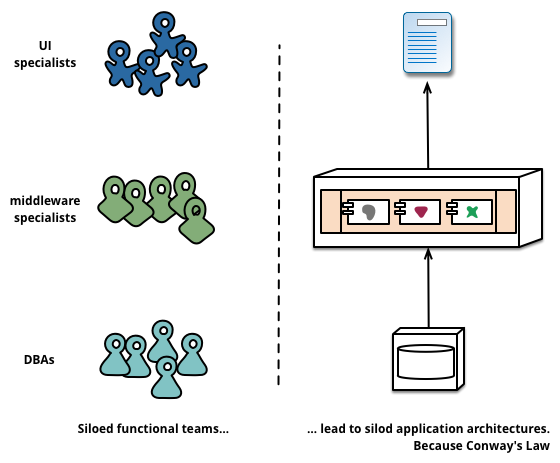
\includegraphics[width=0.8\textwidth]{conways-law.png}
\caption{\label{conway's law}An illustration of Conway's Law}
\end{figure}

This means that the bus is used merely as a message store but does not do any routing or other modification on the messages like a ESB in an SOA would. This helps combine the asynchronism of the SOA with the extreme modularity of a microservice architecture.\\

\subsubsection{Choosing a model}
As stated earlier, each model has its advantages and inconveniences. However, using the SOA was often pointed out as more "beginner friendly" than jumping straight to the microservices model.

We decided to follow the multiple pieces of advice on this subject and start transitioning by implementing an SOA architecture. Indeed it seemed more logical to only divide an application in a couple of services and focus on implementing the communication of the two parts with a bus. There was already some of thought put into what services might ultimately be needed when the transition would be complete, so my mission was mostly to figure out a way to implement this transition on SoMoS II which originally contained the "Production Resources Management", "Production Planning Management" and "Delivery Planning Management" services. 
\begin{figure}[H]
	\centering
	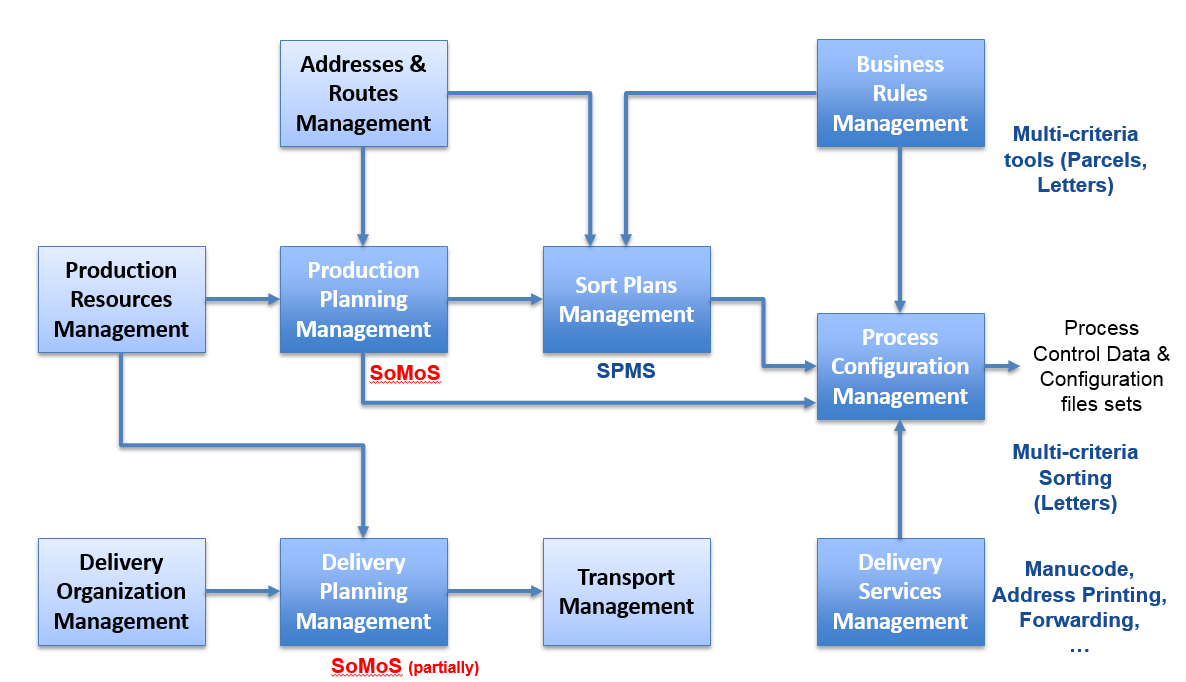
\includegraphics[width=0.8\textwidth]{services.PNG}
	\caption{\label{Solystic service}The different services envisionned by Solystic}
\end{figure}
\subsection{Choosing a product}
With EAI being such a trendy subject among all companies, there exists a plethora of different ESB or similar integration solutions to choose from to implement the expected change in architecture. 
I was however provided with a few constraints. First, the solution found would have to preferably be open source, then it should include a compatibility with a MongoDB database, and finally be reasonably priced and easy to use.

I was able to narrow down my choice to two products among the most popular, due mostly to their relatively easy use even without any experience with middleware or integration in general. Those two products were MuleSoft's AnyPoint Platform and WSO2 Enterprise Integrator. These two products are very similar, for instance they both offer a graphic user interface with which a user can manipulate components and create sequences that translate into XML files. They are also both available "on-location" or in the Cloud. They are also adapted for use in an SOA or a microservice type of system.

Mulesoft's product is used by many major companies, for example Netflix, which during my research has been presented as a leader in terms of microservices implementation. On the other hand, WSO2's solution is used by some government agencies, schools and medical centers around the world. I chose WSO2 Enterprise Integrator, not only because it was fully open source and free to download, but also because the first contact seemed slightly easier. 

Enterprise Integrator (WSO2 EI) joins multiple functionalities. In addition with providing an ESB, it also contains tools to manage Database Services and Business Processes and offers dashboards to monitor the message activity on the ESB. A significant part of my internship was dedicated to discovering and experimenting with this product in order to be more familiar with it and be able to write some documentation about it for future members of this integration project to use. 
\section{Methodology}
\subsection{Global architecture of the solution}
The first step to the separation is to separate the "Production Resource Management" service from the Scenario part of SoMoS II and make the two parts communicate through the ESB. This step is itself divided in substeps:
\begin{enumerate}
	\item Keep the application whole but send the communications between the PRM part and the Scenario part through the ESB
	\item Separate only the classes composing the PRM service but leaving the direct data connexions in the application
\end{enumerate}
\begin{figure}[H]
\centering
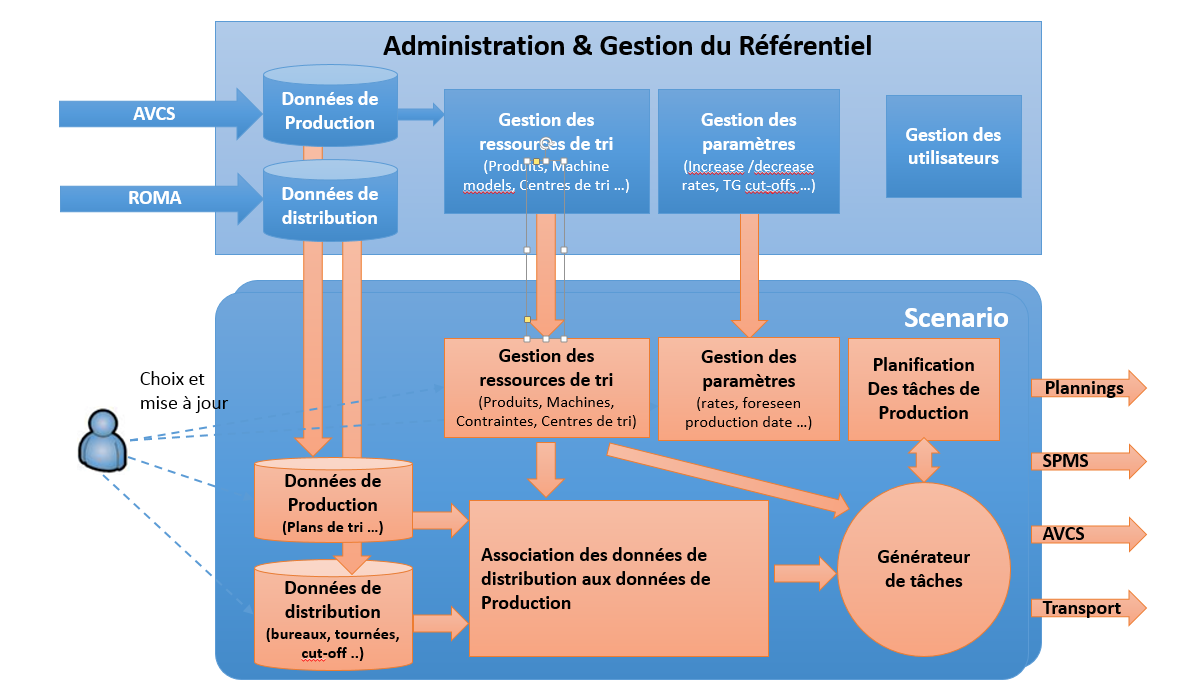
\includegraphics[width=0.9\textwidth]{SOMOS_BASE.PNG}
\caption{\label{basic somos}The basic SoMoS architecture}
\end{figure}

\begin{figure}[H]
\centering
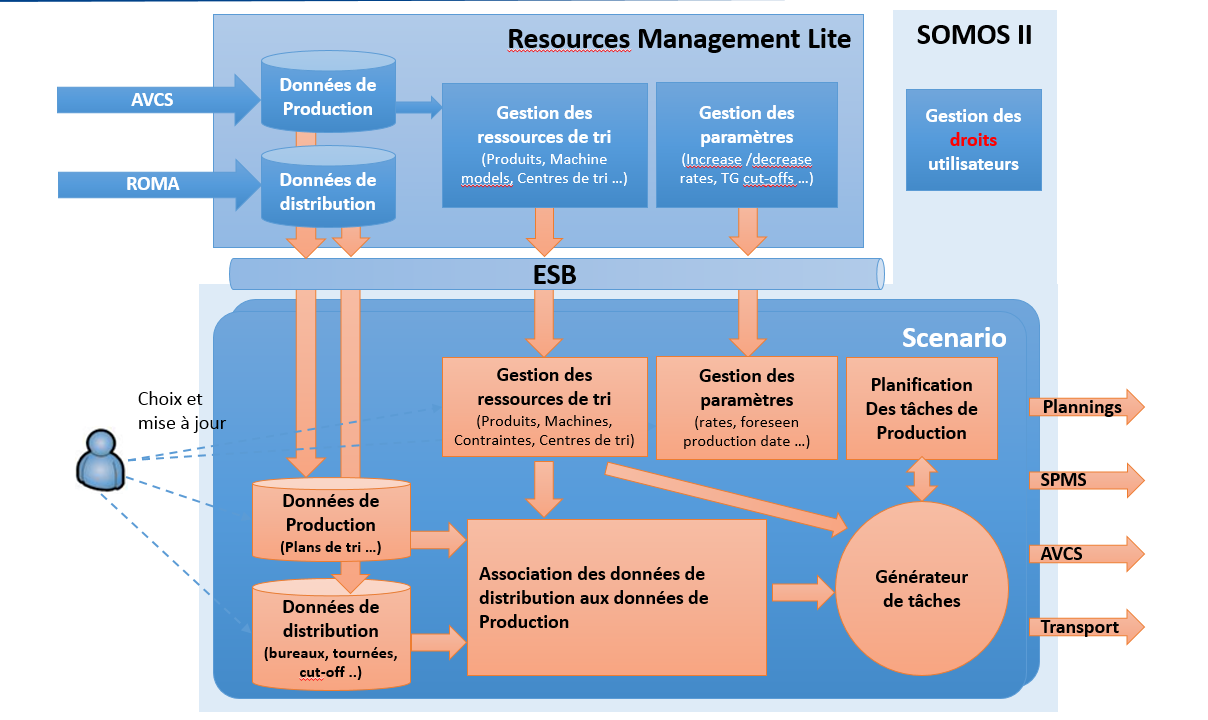
\includegraphics[width=0.9\textwidth]{SOMOS_END2.PNG}
\caption{\label{somos end}The direction in which the project is going}
\end{figure}
\subsection{Detailed implementation}
To achieve this separation, we first need to know where the link between the Production Resources Management (PRM) and the Scenario Management part is situated.

To do this I needed to closely examine the source code of the application. The application is built following a Model, View, Controller architecture. My first instict was then to examine the controllers, and most specifically the Scenario controller. There, and then in the other controllers I found which URLs the ESB needed to connect with, using the \texttt{@Route} markers. I was intending to make the communications possible via HTTP as some controller functions already produced a \texttt{Response} type result when called.

Looking through the Model classes, one PRM-to-Scenario link stood out to me in a \texttt{ScenarioManager} class. Indeed, this class contained the methods to create, view, edit and delete the scenarios and link them to the SoMoS database. The \texttt{build} function gets the Production Resource data from the AVCS and RoMA databases using methods completely equivalent to the ones used in the controller classes. In the \texttt{ScenarioManager} class I created a new function \texttt{getFromESB} that utilizes the cURL lib present with PHP 7 to send a request through the ESB to get the data using the URLs found earlier.

In the ESB, I created an API resource that forwards the \texttt{GET} request to the desired controller and then sends back the \texttt{Response} with a JSON message payload. The function then returns a list of objects that can be used in the \texttt{build} function derived from this JSON payload. If the payload did not exist or was not valid, the function would return an empty list.
Unfortunately, every attempt to create a Scenario using \texttt{getFromESB} resulted in a redirection to the login page and an empty Scenario even though the PRM databases were properly initialized with a set of test values.\\
As the Users Management part was not supposed to be affected by the project I spent little time studying it during my first examination of the source code, meaning that with the little time I had left, I would not risk modifying the user rights to access the services directly without having to go through the login step. And in the long run the same problem would have come up again as it would be unthinkable to produce an application with absolutely no credentials asked to access this type of data.
To fix this issue, i tried to add a new endpoint connecting the ESB to the \texttt{login} or \texttt{login\_check} page before going to the designated URL in order to pass the credentials using a \texttt{POST} request as I learned from the Symfony documentation was the procedure when a login occurred. These attempts did not work either and the messages were lost in between endpoints. 

I was unable to go past this obstacle which means the separation is not complete to this day. My supervisor mentioned the possible need to shift the user rights management to a centralized login procedure, which was not in the scope of the project.
\section{Testing the system and visualizing the results}
\subsection{A first simple application to learn how WSO2 EI works}
Before going to the main subject of this project, i was given a first small application to start familiarizing myself with WSO2 EI as well as testing how much workload it could handle. \\
\begin{figure}[H]
\centering
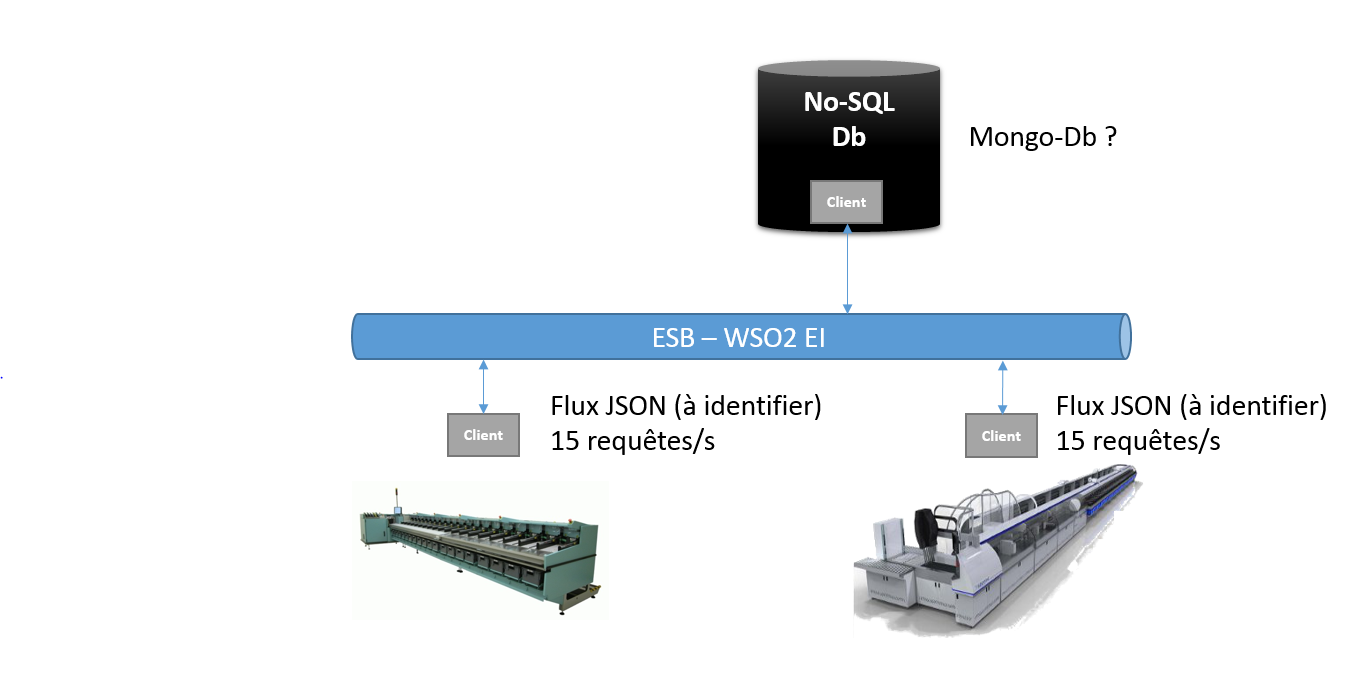
\includegraphics[width=0.9\textwidth]{mini_projet.PNG}
\caption{\label{training maquette}The WSO2 EI training project given by Solystic}
\end{figure}


A given number of sorting machines need to send data about parcels to a database. An example of the type of message produced by a machine is given in the Appendix. The only information that needs to be saved to the database are the values of the \texttt{PracelId} and the \texttt{MachineId} fields. A full explanation on how WSO2 EI was configured to achieve this result is included in the Appendix. 

To test if this a configuration works, I needed to:
\begin{itemize}
\item Allow tracking on the API, the proxy services, the sequence and all the endpoints
\item Activate the Analytics profile
\item Have a means to simulate a machine sending a message to the API
\end{itemize}

This last point is the one that varies according to which property is tested.

To test if a message sent by the machine reaches the desired endpoint, i used cURL with the verbose option, as only one message needed to be sent. After receiving an OK response via cURL, I could also verify that the message did indeed pass through all the intended services, endpoints and sequences to the database using the Analytics dashboards. From this display, I could check the changing payload and acceptance from the Database service.

When the system is correctly configured, it is time to test how much workload one entity can handle. At first i tried to set VMs as message senders, to simulate the fact that multiple machines are actively soliciting the system. This could have been possible but such a setup needed the installation of a third party load balancer and further configurations. Time constraints discouraged me from attempting to install and learn about yet again one new voluminous tool on my own. 

My supervisor introduced me to a testing tool that Solystic uses regularly : Apache JMeter. After configuring the tool to send from 5 threads to the service at a rate of 15 messages per second for approximately 10 seconds at a time, I could view the results via WSO2 Analytics, this time focusing on the Requests per second panel. The 75 messages per second were handled correctly. However, if the workload was doubled, with 10 threads instead of 5 working at 15 messages per second, the ESB peaks at 85 messages processed per second even if the message processor was configured to be able to handle up to 500 messages at a time.
%using regular cURL\\
%trying to use a VM\\
%using JMeter
\subsection{Trying to test the project solution attempt}
After making the modifications on SoMoS II and configuring the ESB, I deployed the SoMoS application on the Apache server, activated the Analytics profile of WSO2 EI and attempted to create a Scenario using default values. After the application marked the Scenario as completed, I checked the values of the different production resources fields only to find them all at the N/A value. That means the value of the \texttt{Response} awaited by \texttt{getFromESB} was either non-existent or invalid. When checking WSO2 Analytics, the message was marked as successfully transmitted but it was not possible for me to see the payload of the response sent by the service. 
Trying to contact the ESB with a simple in-terminal cURL command showed me that the message was redirected towards to the login page.

After applying the "patch" described earlier, i.e. trying to pass the message to the login page BEFORE changing it in the ESB and sending it to the service, I ran the same tests in the same order. Attempting to create a Scenario via the SoMoS II application still prompted an empty Scenario in the system. Checking Analytics yielded a rather surprising result: there was no trace of the passage of the message through the ESB even after checking thouroughly that tracing had been enabled on every component of the system. Running an in-terminal cURL command returned an "empty response from server" type of error. 

\section{Personal Record}
\subsection{First professional experience}
This was my first internship and I was somewhat intimidated by the environment. I did work alone, as the members who worked on the SoMoS II application were situated in Bagneux and I was in Bourg-lès-Valence. My only regular contacts in the company were my supervisor and the SoMoS project manager whom I contacted via e-mail or phone whenever i had a question about the application.

This did not help with my integration in the department, even though i was present for 3 months and a half. That combined with personal problems, I could say that my personal daily experience could have been better.  
\subsection{Working with new tools}
All the tools and environments used in this internship were new or unfamiliar to me. Firstly, working in a Windows environment was somewhat destabilizing as I was used to work at school as well as at home on Linux operating systems. Then, the concept of Enterprise Application Integration was entirely unknown to me, as I was used to thinking about software architecture on a smaller scale. Not only that, but the products I had to test (in particular WSO2 EI) were new to the company too, so any help that I needed I had to look for myself on WSO2 documentation or other sources.

Concerning SoMoS II, I was not familiar at all with the PHP language but my knowledge of object oriented programmation helped me understand the syntax and structure of the application. This sadly was not enough to help me understand the inner workings 
of Symfony's security system and fix the login issue I encountered.

I was also introduced to corporate working tools such as RedMine and SVN, useful for versioning and assigning missions. I did not get a lot of use of these except for the redaction of a short Wiki article explaining how to install and understand WSO2 EI through the simple training application i developed in the first half of the internship.

This lack of prior knowledge of any of the elements I used in this internship did make my work slow, as i had to review the basics and read a lot of documentation. It might be one of the reasons why the objectives of this internship were not met.
\subsection{Supervising a student}
During the last week, I was introduced to a first year Ensimag co-op student who will be continuing the project started during this internship and pushing further the transition to the new architecture model. Helping her get started with the different tools used in the company, or that I introduced helped me visualize better the amount of knowledge i have aggregated during this experience.
\section{Conclusion}
As a conclusion, even though this intership's goal was not met, it was still a tremendously enriching experience. Indeed, I gathered new knowledge and skills that i did not obtain through my school education. This experience did help me to explore beyond my comfort zone and to push my limits. I was honored to be tasked with a mission with this much responsibility even if my skills might not have lived up to the company's expectations.   
\newpage
\part*{Appendices}
\section*{Glossary}
\begin{enumerate}
\item \textbf{EAI:} Enterprise Application Integration. A type of architecture in which different applications are connected.
\item \textbf{SOA:} Service Oriented Architecture. A model that is part of EAI and consists in a number of services communicating through a bus.
\item \textbf{ESB:} Enterprise Service Bus. A piece of middleware that transfers, routes and sometimes modify messages from one service to another.
\item \textbf{PRM:} Production Resources Management. One of the services contained in the current SoMoS II application. It helps manage (view, edit create and delete) the sorting types, sorting sites, machines, sorting parameters and the machine characteristics.
\item \textbf{WSO2 EI:} WSO2 Enterprise Integrator. WSO2's integration solution. It includes an ESB, a Message Broker that helps manage message queues and message consumers, a Data Service Server, and an Analytics profile that is useful for monitoring the messages going through the system.
\end{enumerate}
\section*{References}
\begin{itemize}
	\item \href{https://eclass.upatras.gr/modules/document/file.php/EE653/\%CE\%95\%CF\%81\%CE\%B3\%CE\%B1\%CF\%83\%CE\%AF\%CE\%B5\%CF\%82/Integration\%20of\%20Distributed\%20Enterprise\%20Applications_A\%20Survey.pdf}{\textit{Integration of Distributed Enterprise Applications: A Survey} - Wu He, Li Da Xu (2011)}
	\item \href{https://martinfowler.com/articles/microservices.html}{\textit{Microservices} - Martin Fowler (2014)}
	\item \href{https://docs.wso2.com/display/EI611/WSO2+Enterprise+Integrator+Documentation}{WSO2 EI Documentation}
	\item PHP manual
	\item Symfony manual
\end{itemize}
\newpage
\section{The Wiki I wrote on using WSO2 EI}
\begin{figure}[H]
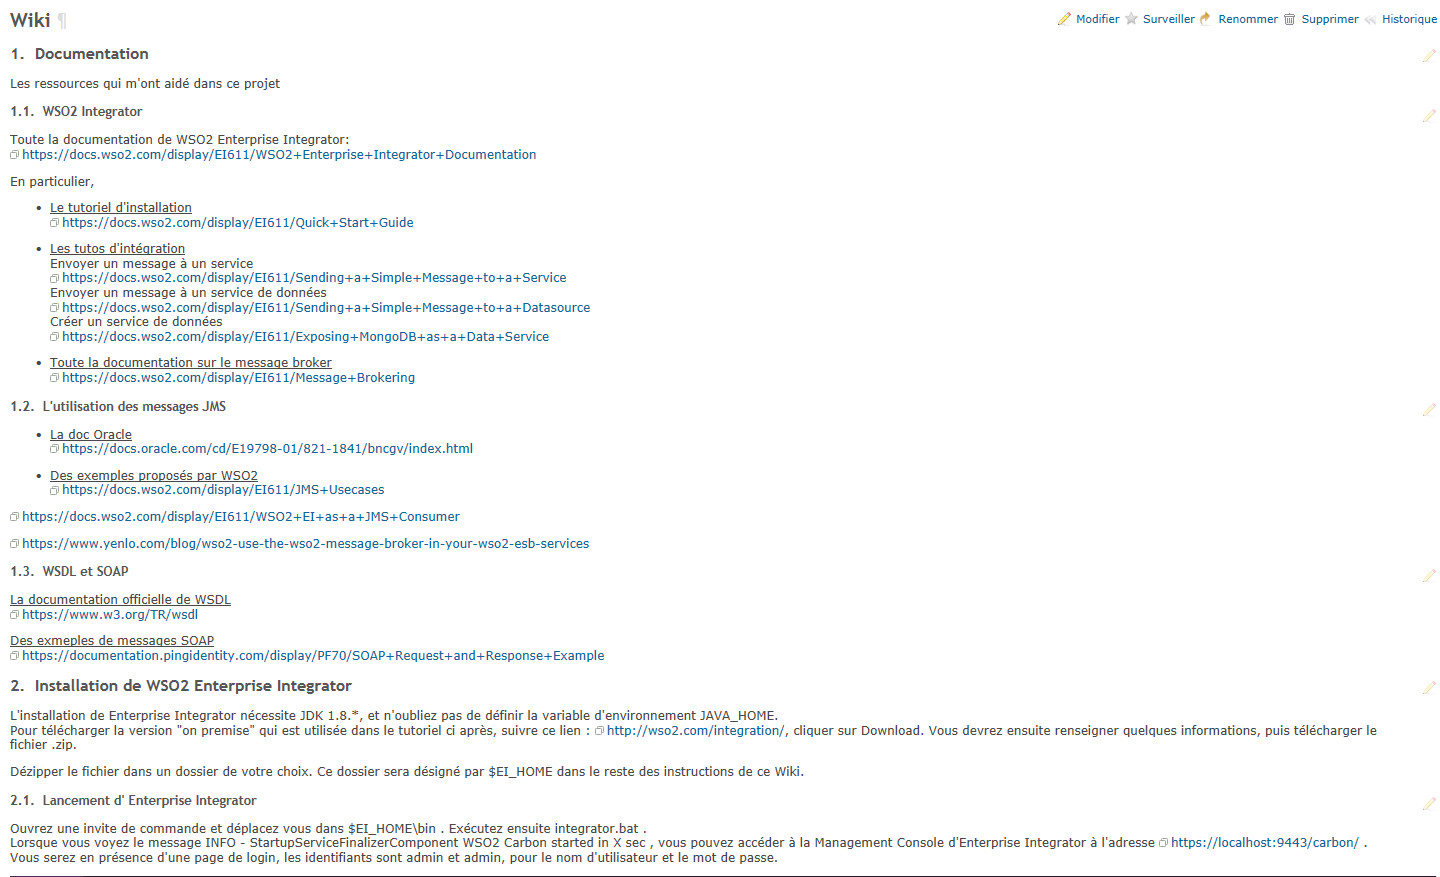
\includegraphics[width=\textwidth, height= 0.45\textheight]{wiki1.PNG}
\end{figure}
\begin{figure}[H]
	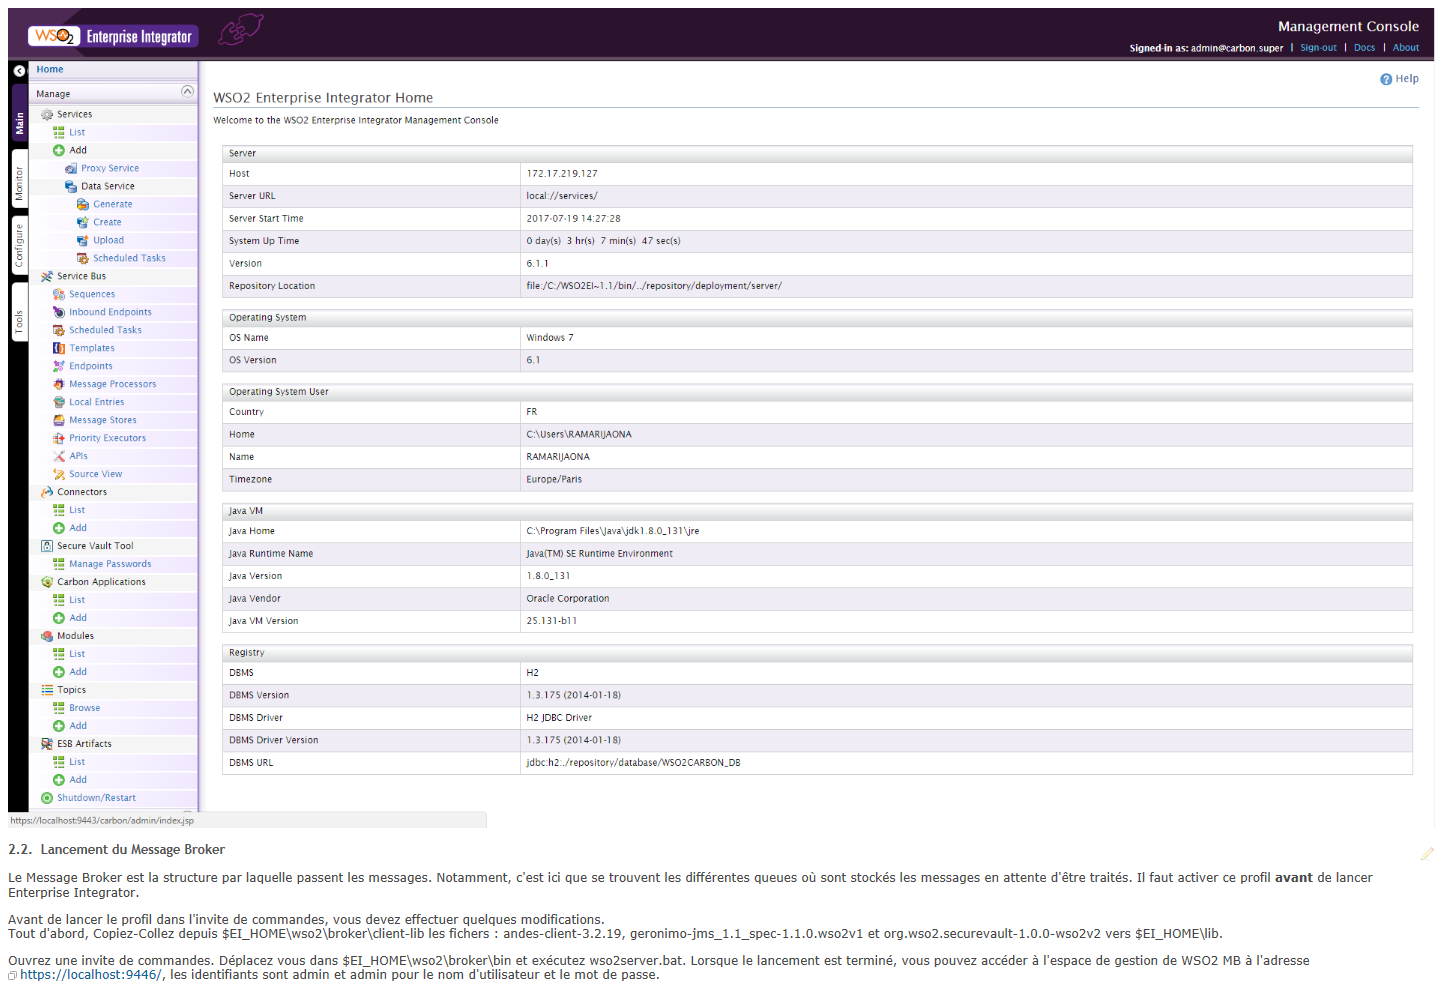
\includegraphics[width=\textwidth, height= 0.45\textheight]{wiki2.PNG}
\end{figure}
\begin{figure}[H]
	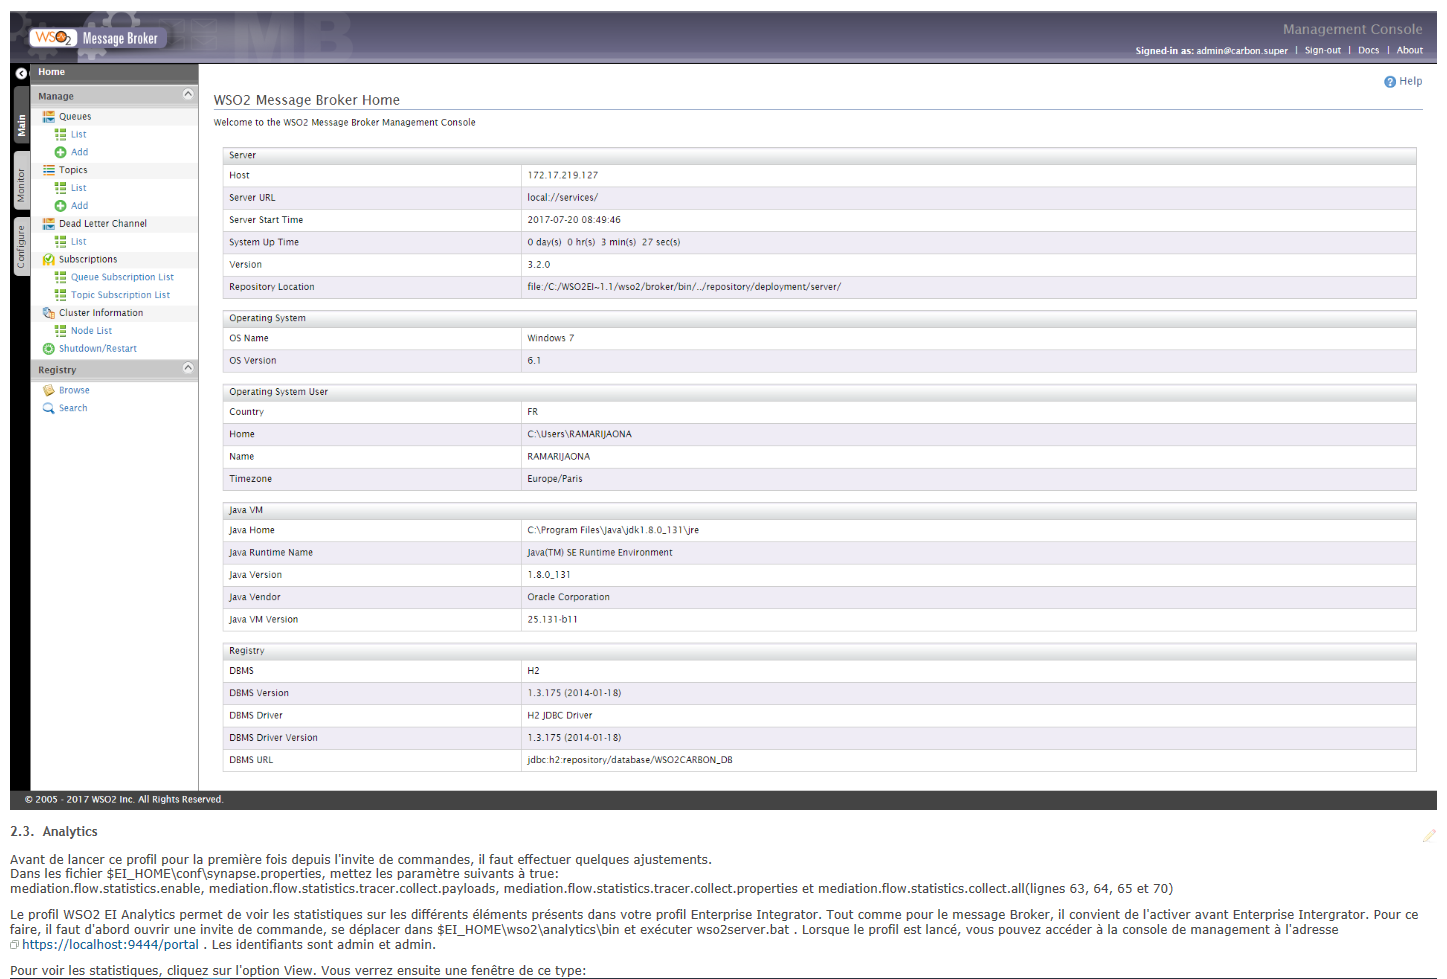
\includegraphics[width=\textwidth, height= 0.45\textheight]{wiki3.PNG}
\end{figure}
\begin{figure}[H]
	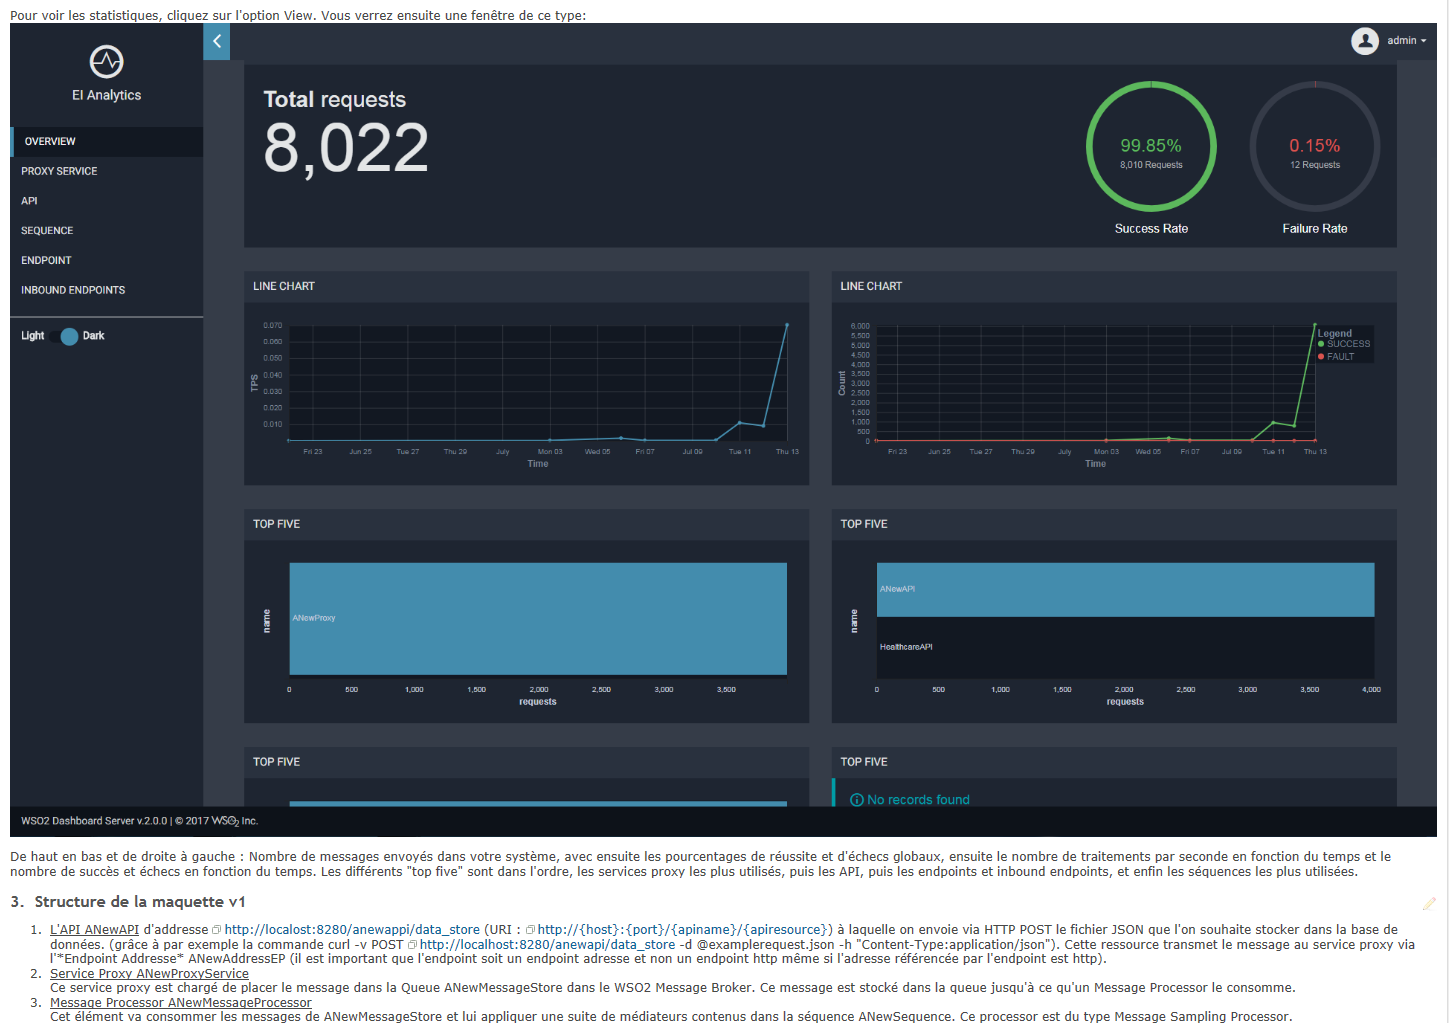
\includegraphics[width=\textwidth, height= 0.45\textheight]{wiki4.PNG}
\end{figure}
\begin{figure}[H]
	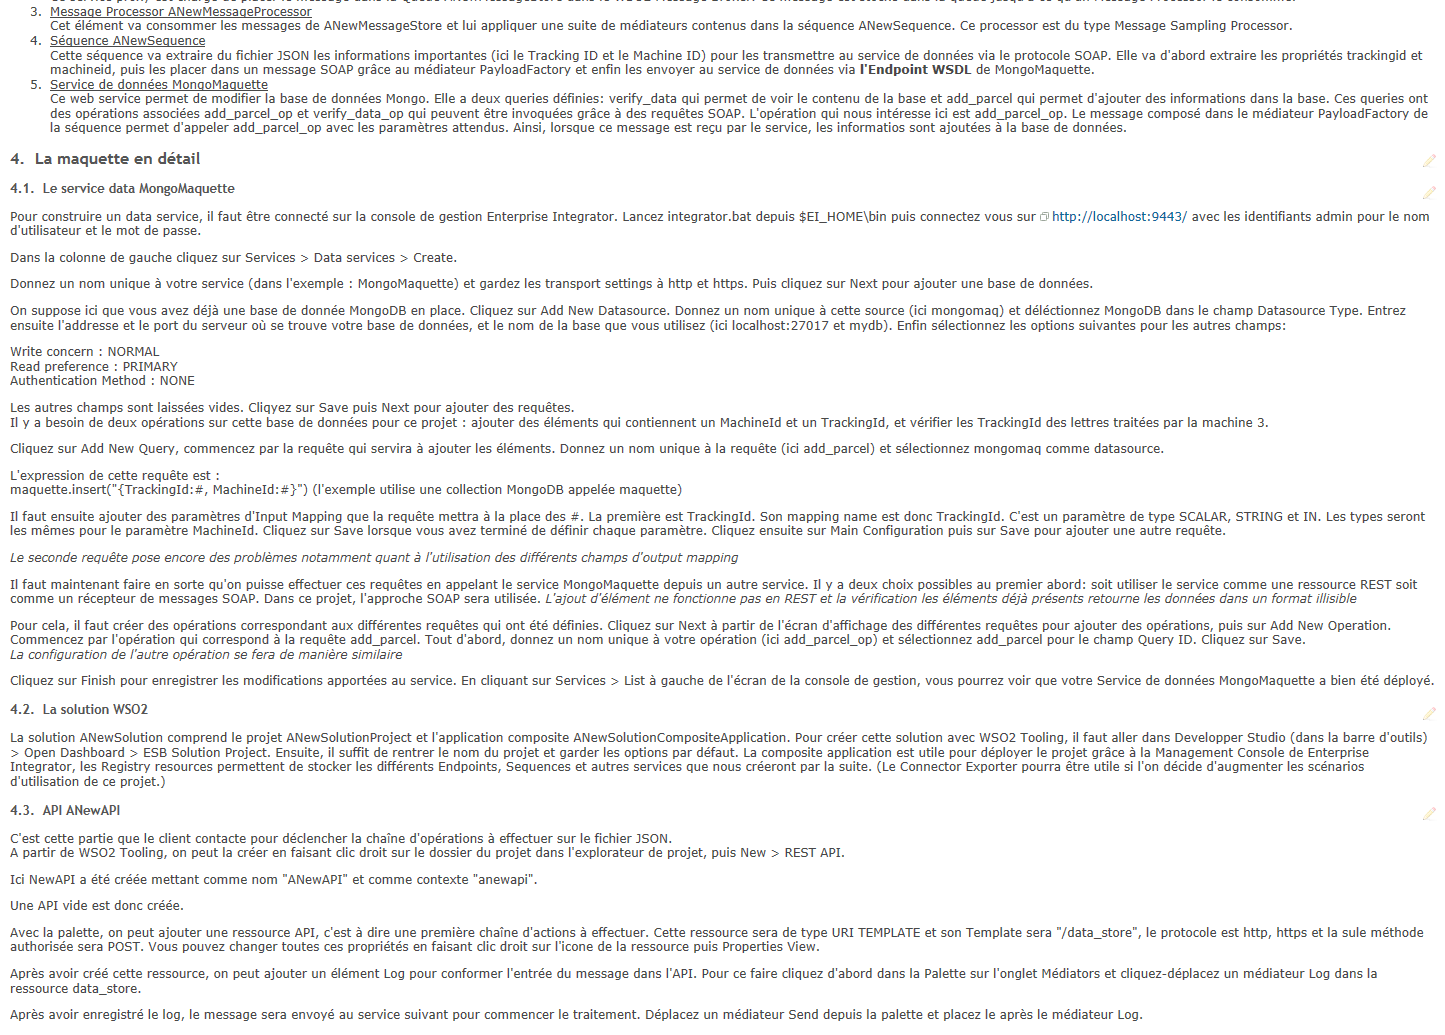
\includegraphics[width=\textwidth, height= 0.45\textheight]{wiki5.PNG}
\end{figure}
\begin{figure}[H]
	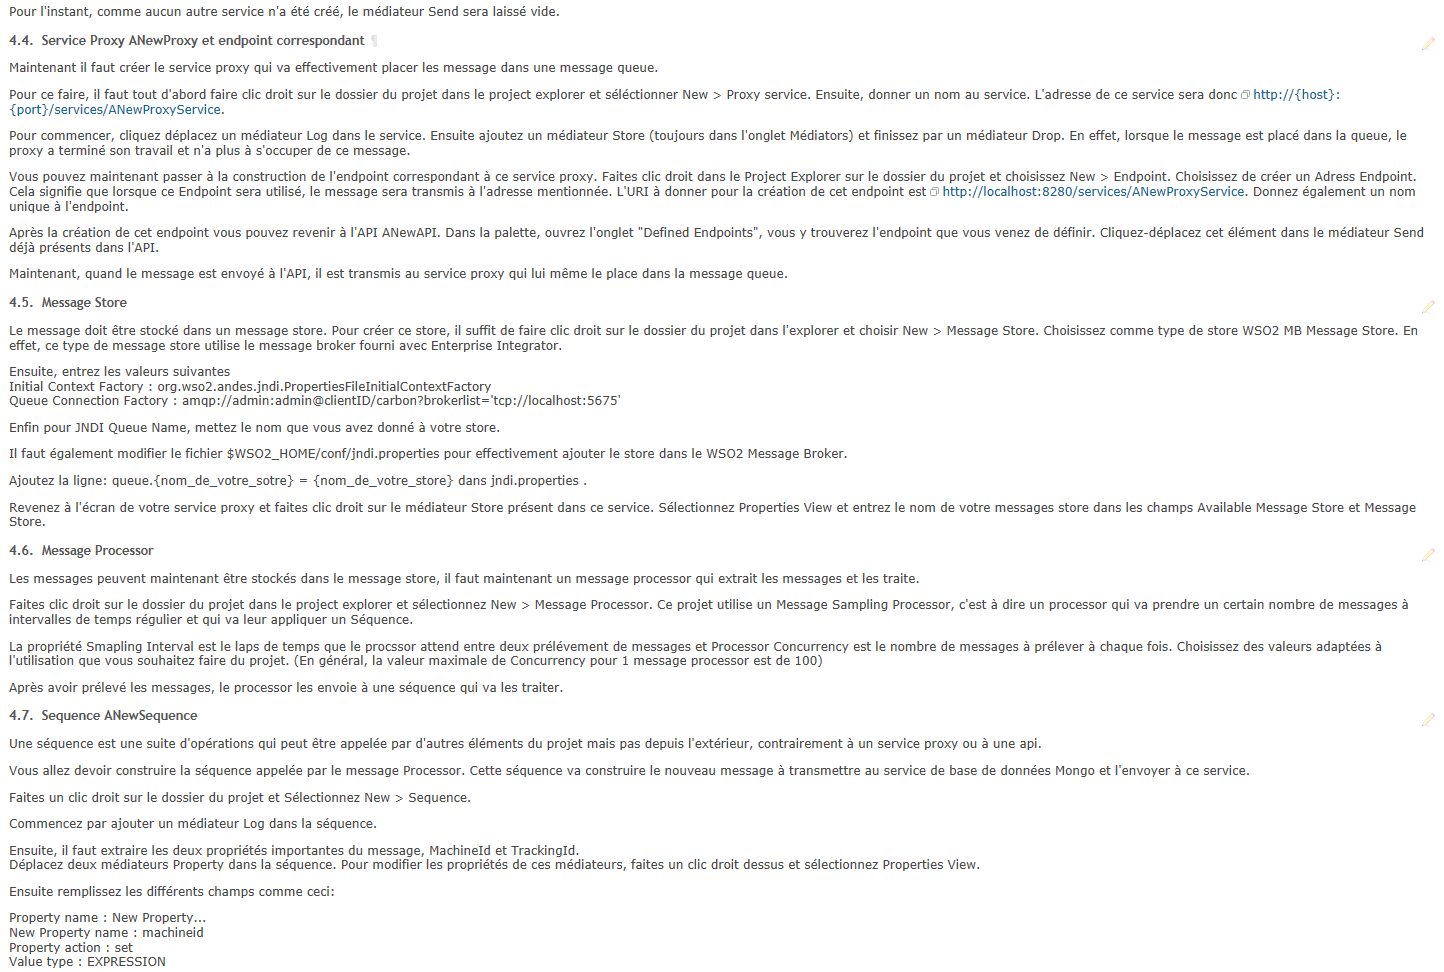
\includegraphics[width=\textwidth, height= 0.45\textheight]{wiki6.PNG}
\end{figure}
\begin{figure}[H]
	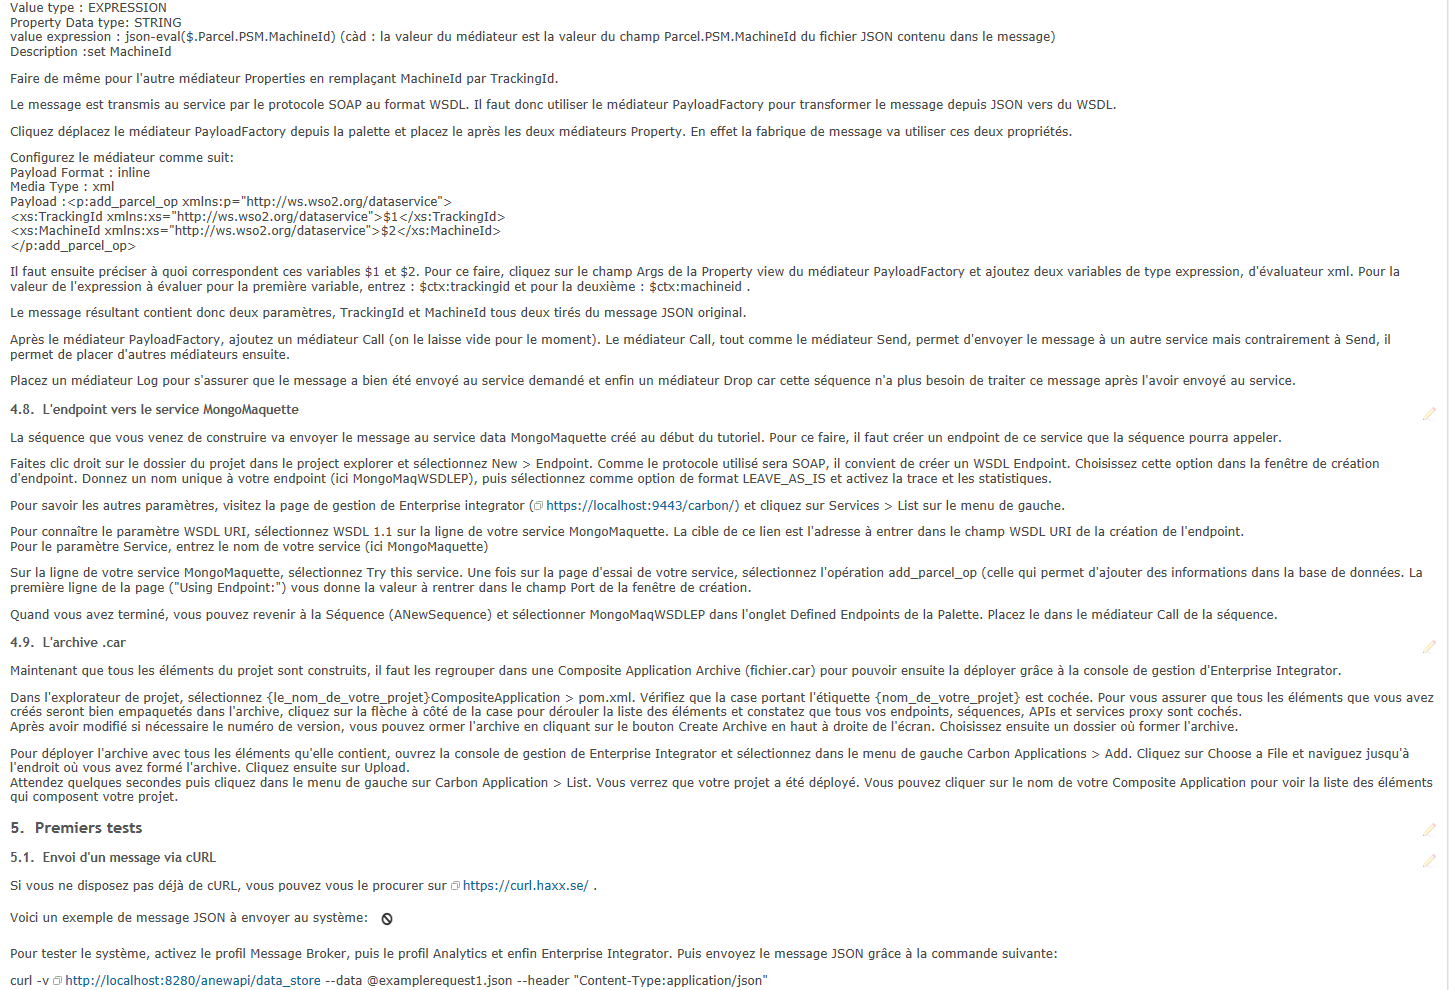
\includegraphics[width=\textwidth, height= 0.45\textheight]{wiki7.PNG}
\end{figure}
\begin{figure}[H]
	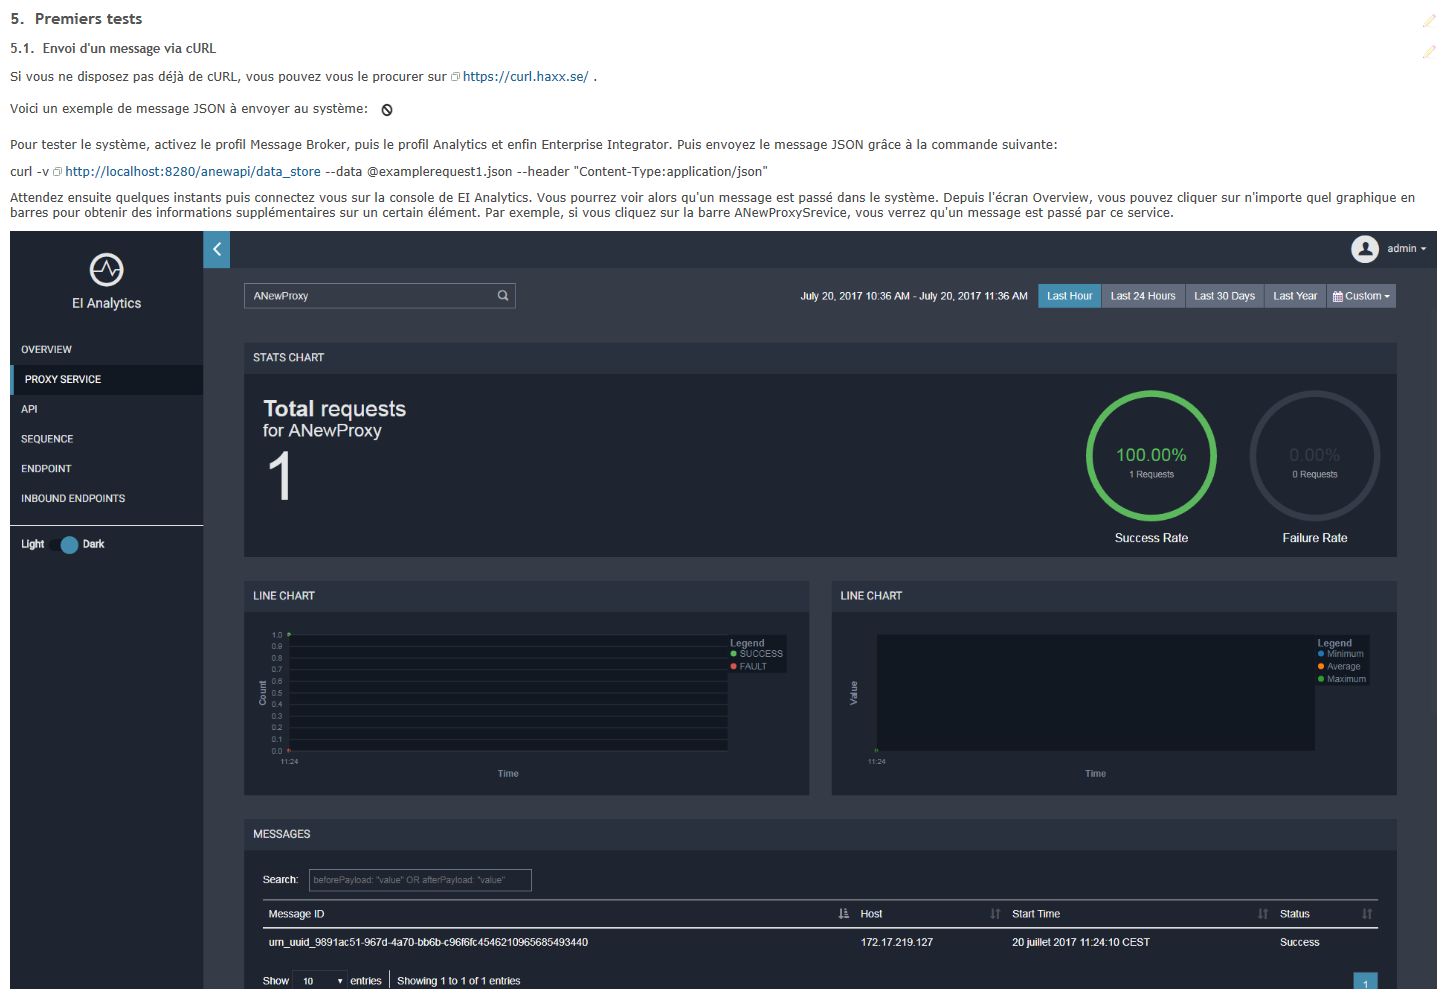
\includegraphics[width=\textwidth, height= 0.45\textheight]{wiki8.PNG}
\end{figure}
\begin{figure}[H]
	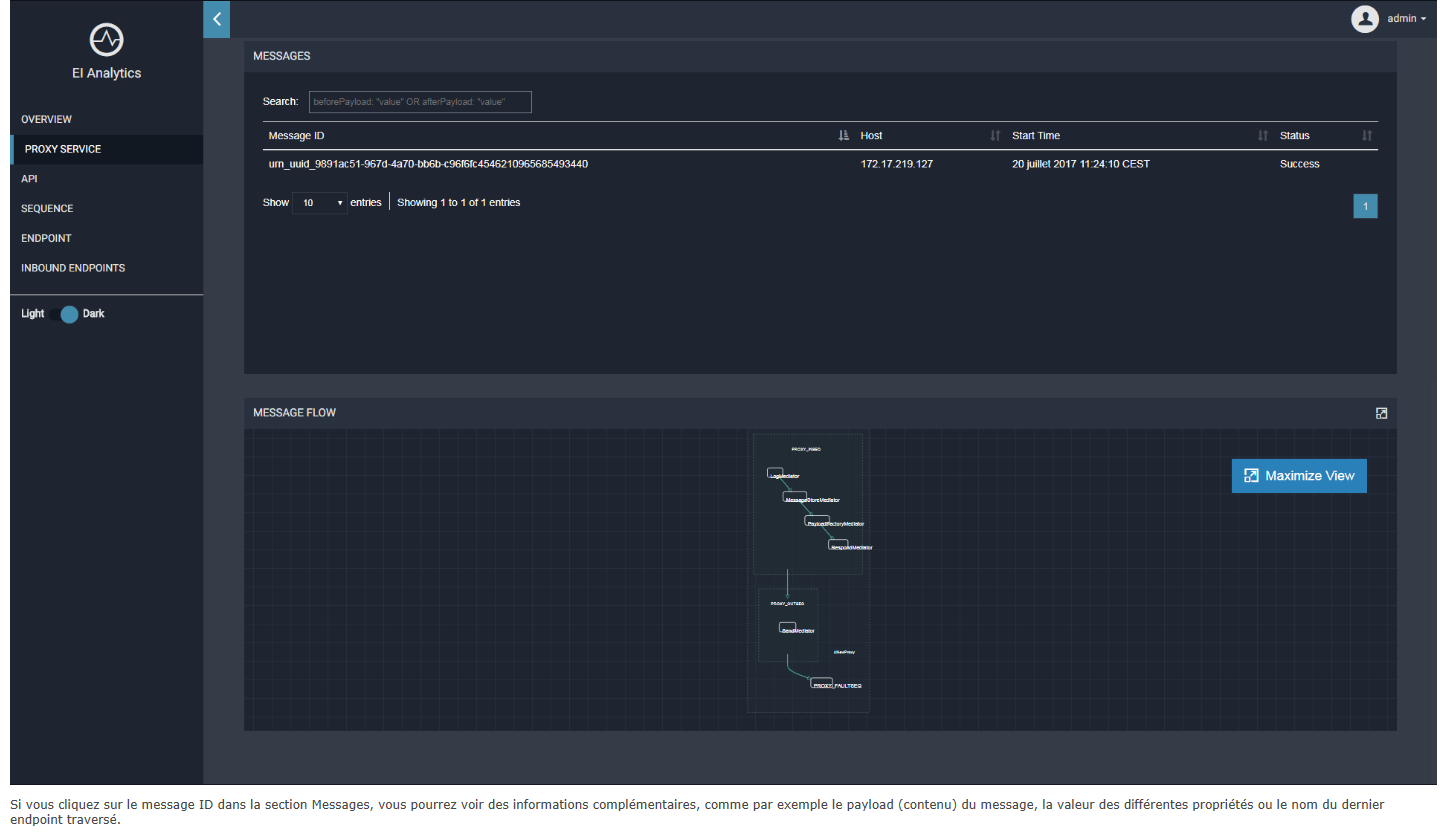
\includegraphics[width=\textwidth, height= 0.45\textheight]{wiki9.PNG}
\end{figure}
\newpage
\section*{Visuals from the SoMoS II application}
\begin{figure}[H]
\centering
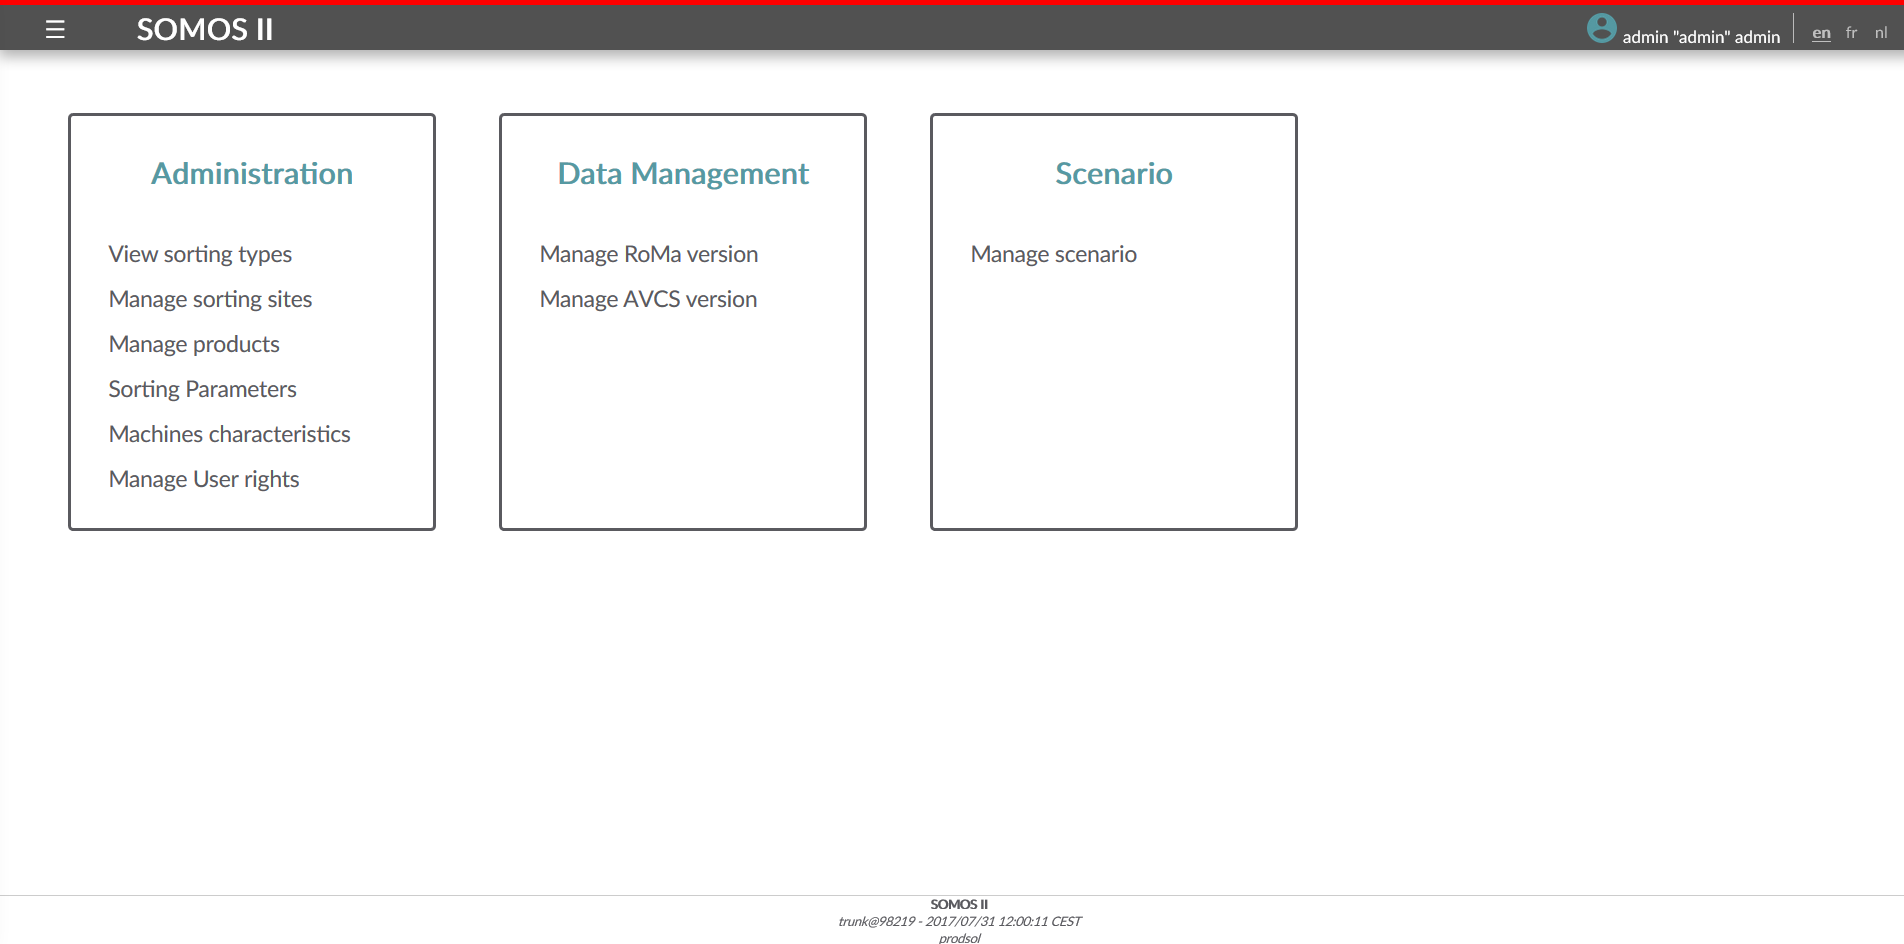
\includegraphics[width=0.8\textwidth]{SOMOS2_1.PNG}
\caption{\label{SOMOS ACCUEIL}SoMoS II Homepage}
\end{figure}
\begin{figure}[H]
	\centering
	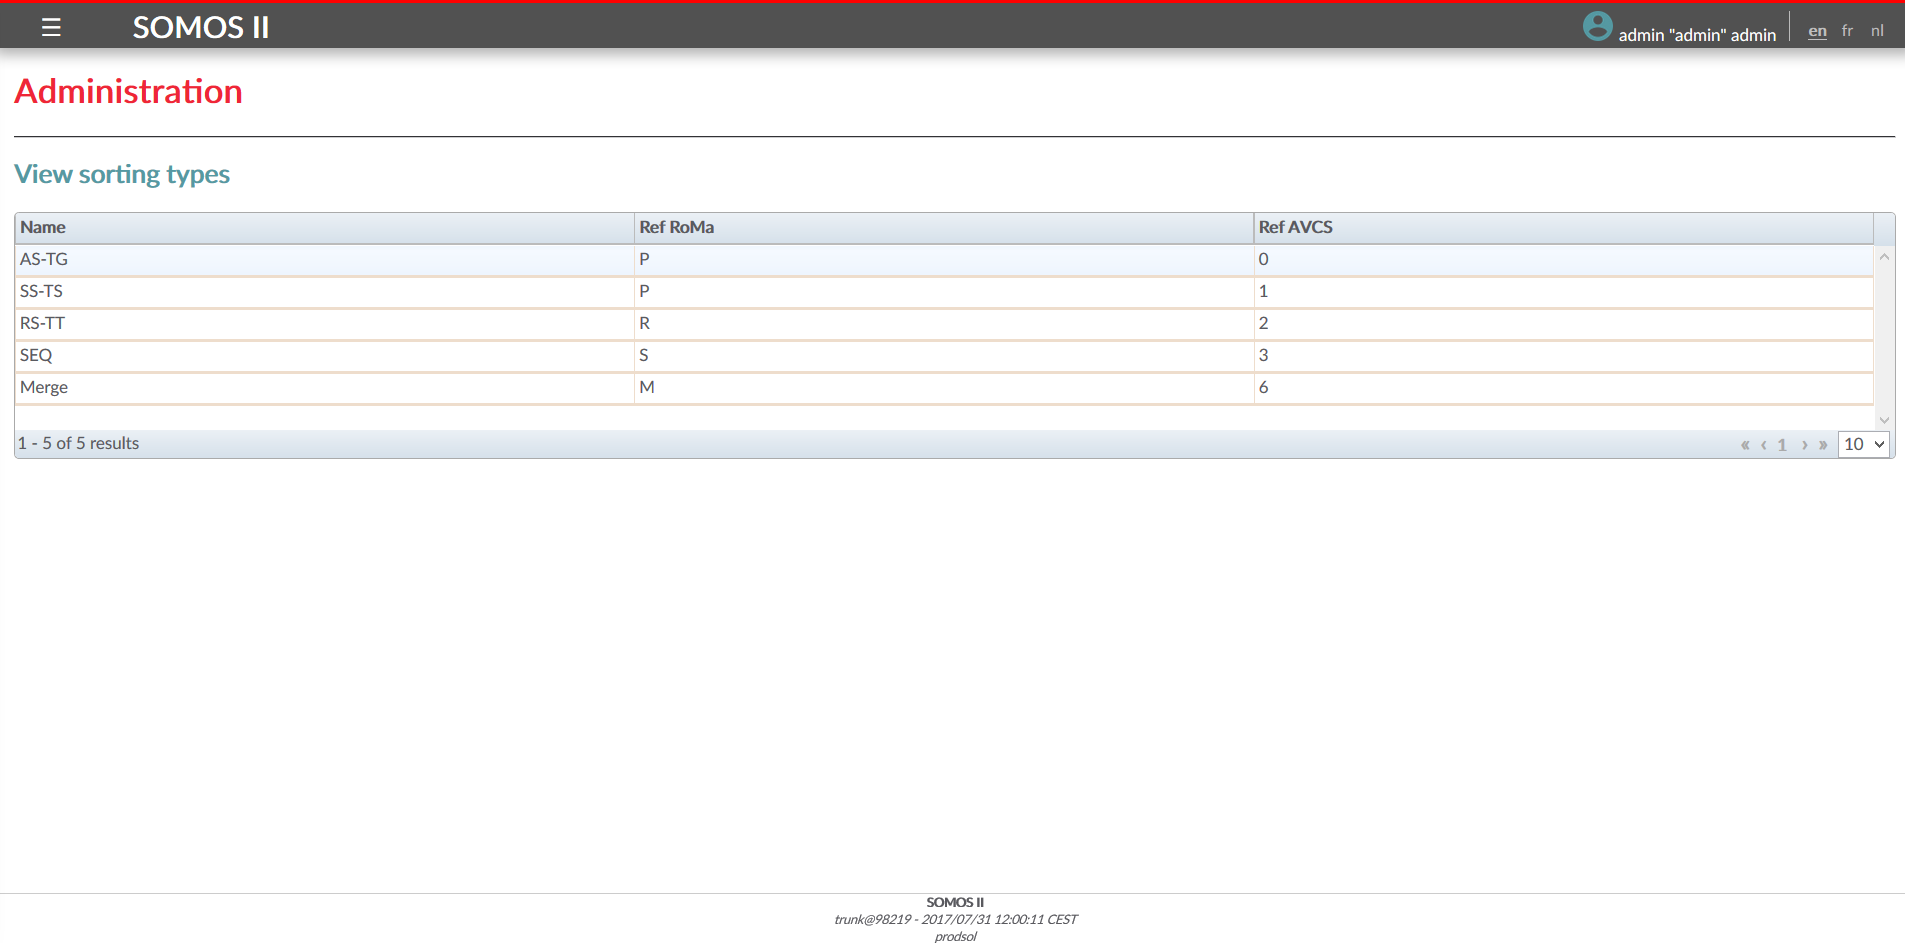
\includegraphics[width=0.8\textwidth]{SOMOS2_2.PNG}
	\caption{\label{SOMOS Sorting Types}A PRM page}
\end{figure}
\begin{figure}[H]
	\centering
	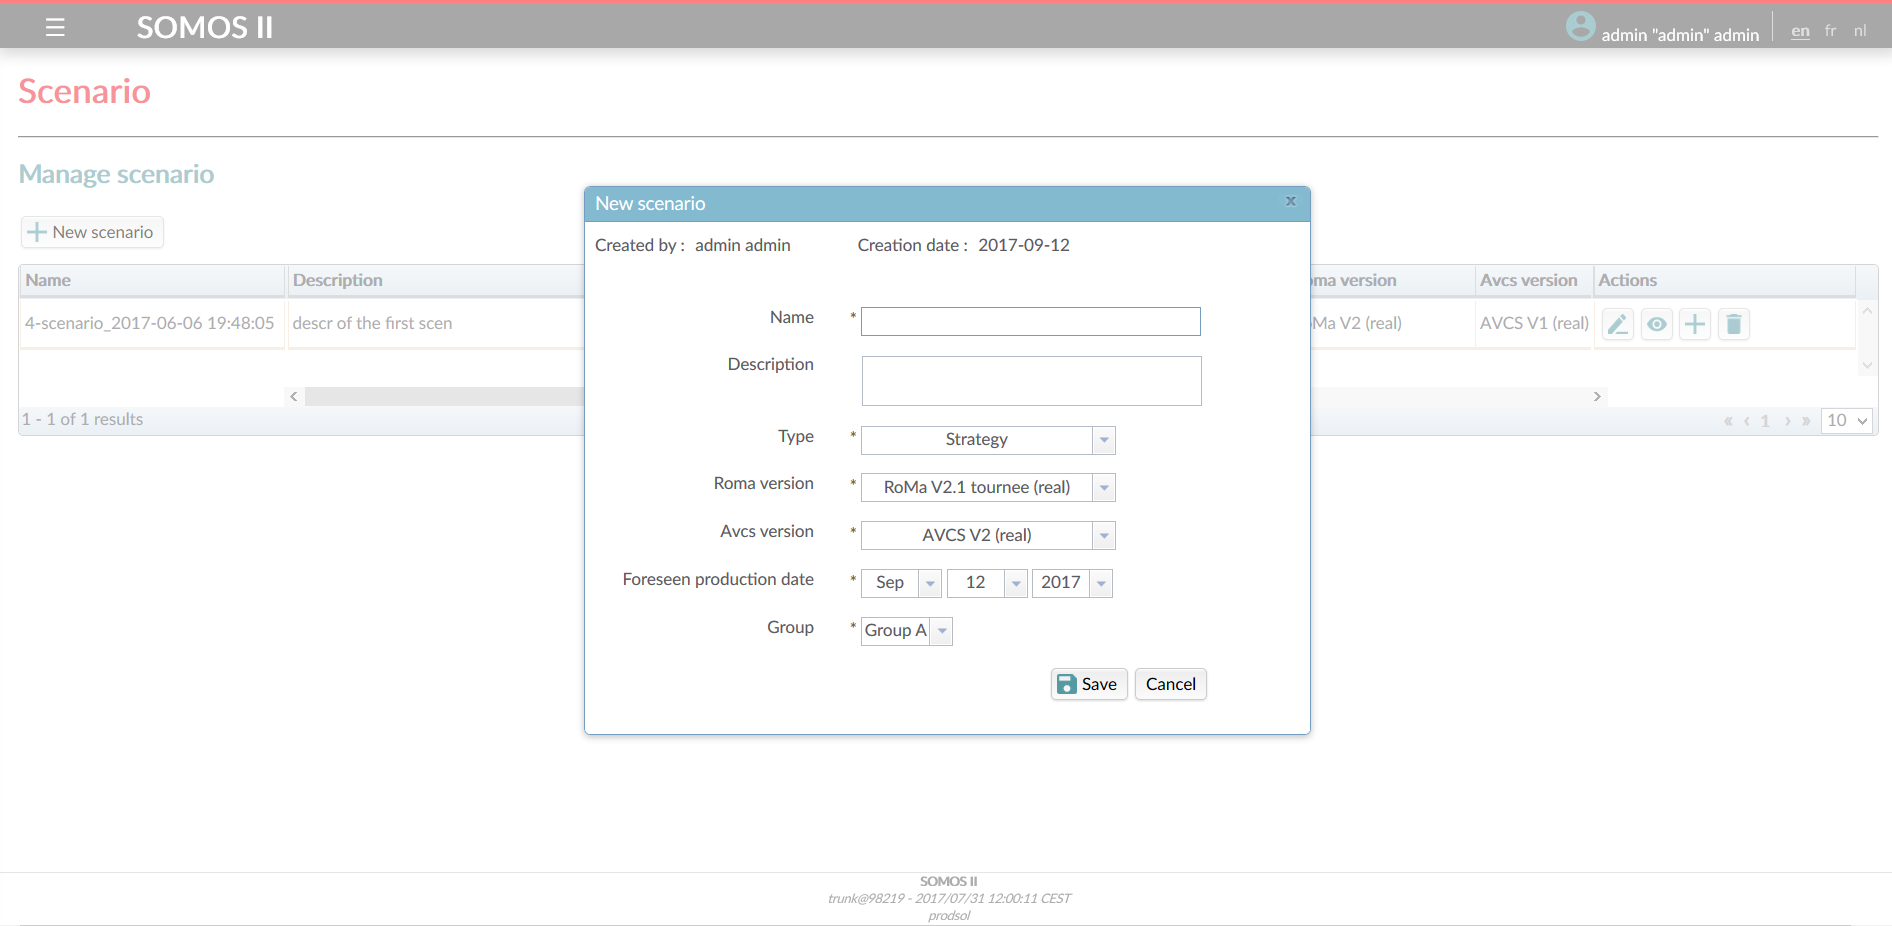
\includegraphics[width=0.8\textwidth]{SOMOS2_3.PNG}
	\caption{\label{SOMOS SCN}Creating a Scenario}
\end{figure}
\newpage

\section*{Visuals from WSO2 Tooling}
WSO2 Tooling is the environment that allows a developer to configure WSO2 EI, to create APIs, proxy services and endpoints (refer to the Wiki to learn more about what these are). Here are some screenshots of the GUI. All of the strucutres shown come from the "training application" that i built to learn about WSO2.

\begin{figure}[H]
\centering
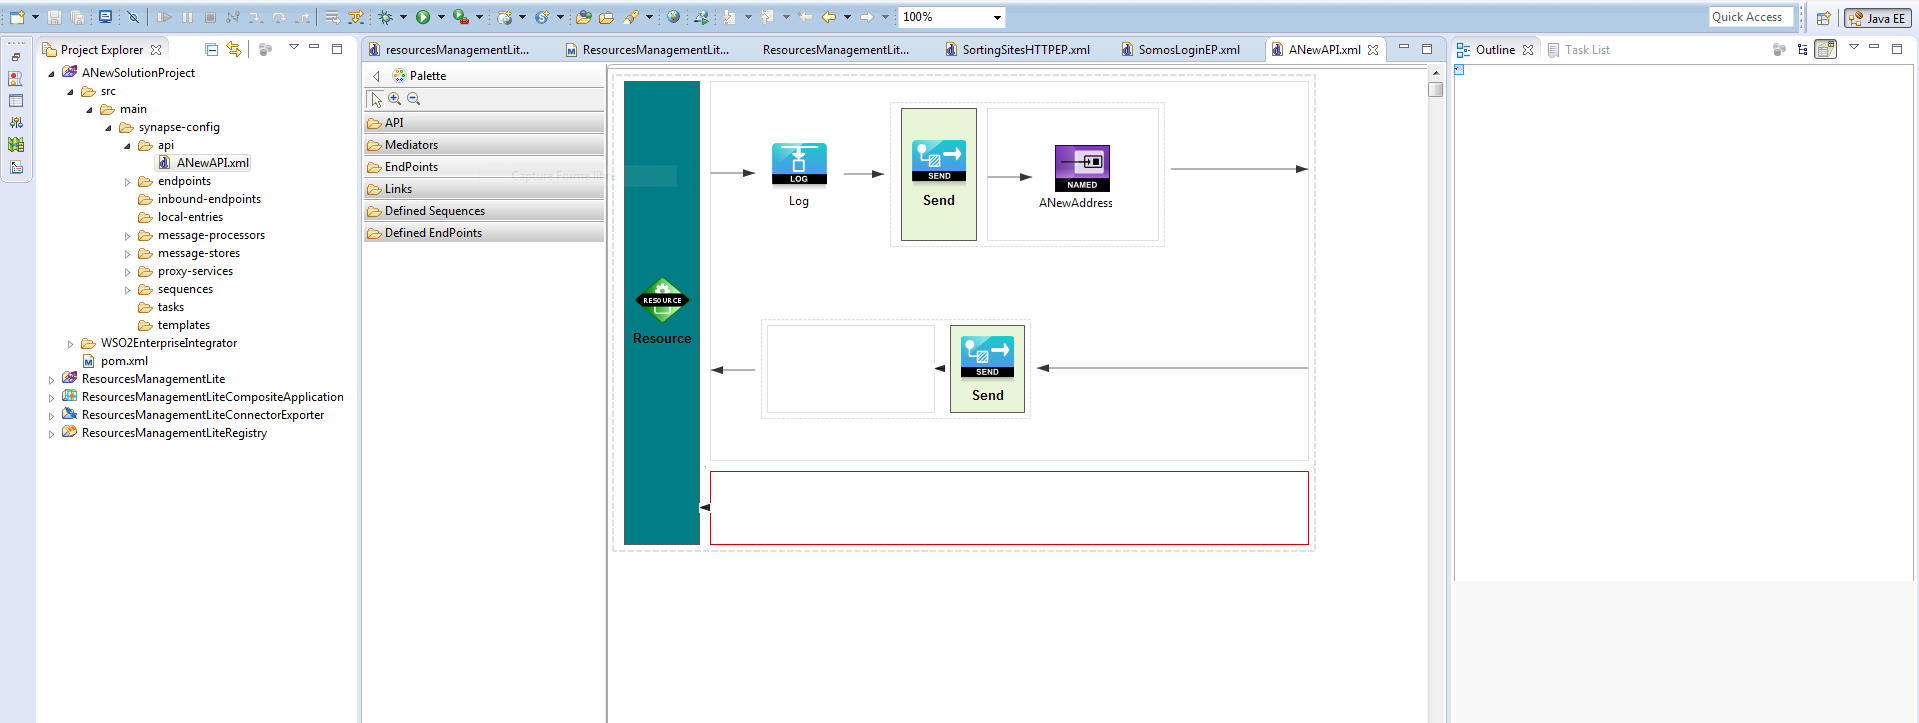
\includegraphics[width=\textwidth]{ESB1.PNG}
\caption{\label{Tooling1}The layout of the GUI (Eclipse based)}
\end{figure}
\begin{figure}[H]
	\centering
	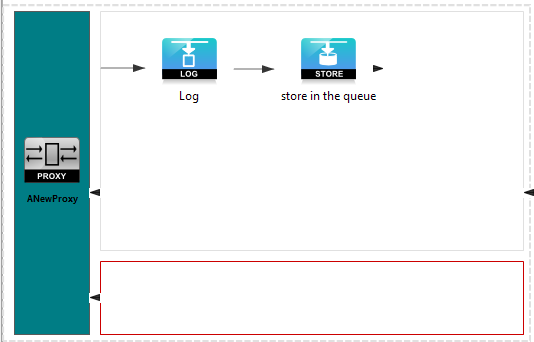
\includegraphics[width=\textwidth]{ESB2.PNG}
	\caption{\label{Tooling2}A service that stores a message in a queue}
\end{figure}
\begin{figure}[H]
	\centering
	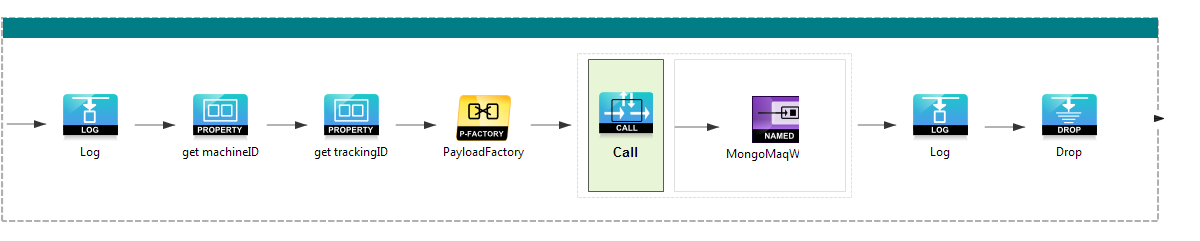
\includegraphics[width=\textwidth]{ESB3.PNG}
	\caption{\label{Tooling3}A sequence}
\end{figure}
% \subsection{How to add Citations and a References List}
%https://eclass.upatras.gr/modules/document/file.php/EE653/%CE%95%CF%81%CE%B3%CE%B1%CF%83%CE%AF%CE%B5%CF%82/Integration%20of%20Distributed%20Enterprise%20Applications_A%20Survey.pdf <- it's a source
% You can upload a \verb|.bib| file containing your BibTeX entries, created with JabRef; or import your \href{https://www.overleaf.com/blog/184}{Mendeley}, CiteULike or Zotero library as a \verb|.bib| file. You can then cite entries from it, like this: \cite{greenwade93}. Just remember to specify a bibliography style, as well as the filename of the \verb|.bib|.

% You can find a \href{https://www.overleaf.com/help/97-how-to-include-a-bibliography-using-bibtex}{video tutorial here} to learn more about BibTeX.

% We hope you find Overleaf useful, and please let us know if you have any feedback using the help menu above --- or use the contact form at \url{https://www.overleaf.com/contact}!

% \bibliographystyle{alpha}
% \bibliography{sample}

% \begin{figure}
% \centering
% 
\includegraphics[width=0.3\textwidth]{frog.jpg}
% \caption{\label{fig:frog}This frog was uploaded via the project menu.}
% \end{figure}

% \begin{table}
% \centering
% \begin{tabular}{l|r}
% Item & Quantity \\\hline
% Widgets & 42 \\
% Gadgets & 13
% \end{tabular}
% \caption{\label{tab:widgets}An example table.}
% \end{table}

% \begin{enumerate}
% \item Like this,
% \item and like this.
% \end{enumerate}
% \dots or bullet points \dots
% \begin{itemize}
% \item Like this,
% \item and like this.
% \end{itemize}
\end{document}